\section{Drift Chambers (DC)}

\subsection{Geometry}

The FTOF geometry is implemented through the COATJAVA geometry service.
The service provides the geant4 definitions that are read by the GEMC perl api to build the geometry database.

Each layer is a generic G4Trapezoid, tilted by $+6^O$ or $-6^O$ depending if they are part of a stereo superlayer or not.
The 12 layers in each region (6 per superlayer) are placed in a region mother volume made of air, see \F{dcGeometry}.
The wire identifications is performed in the Process ID routine.

\begin{figure}
	\centering
	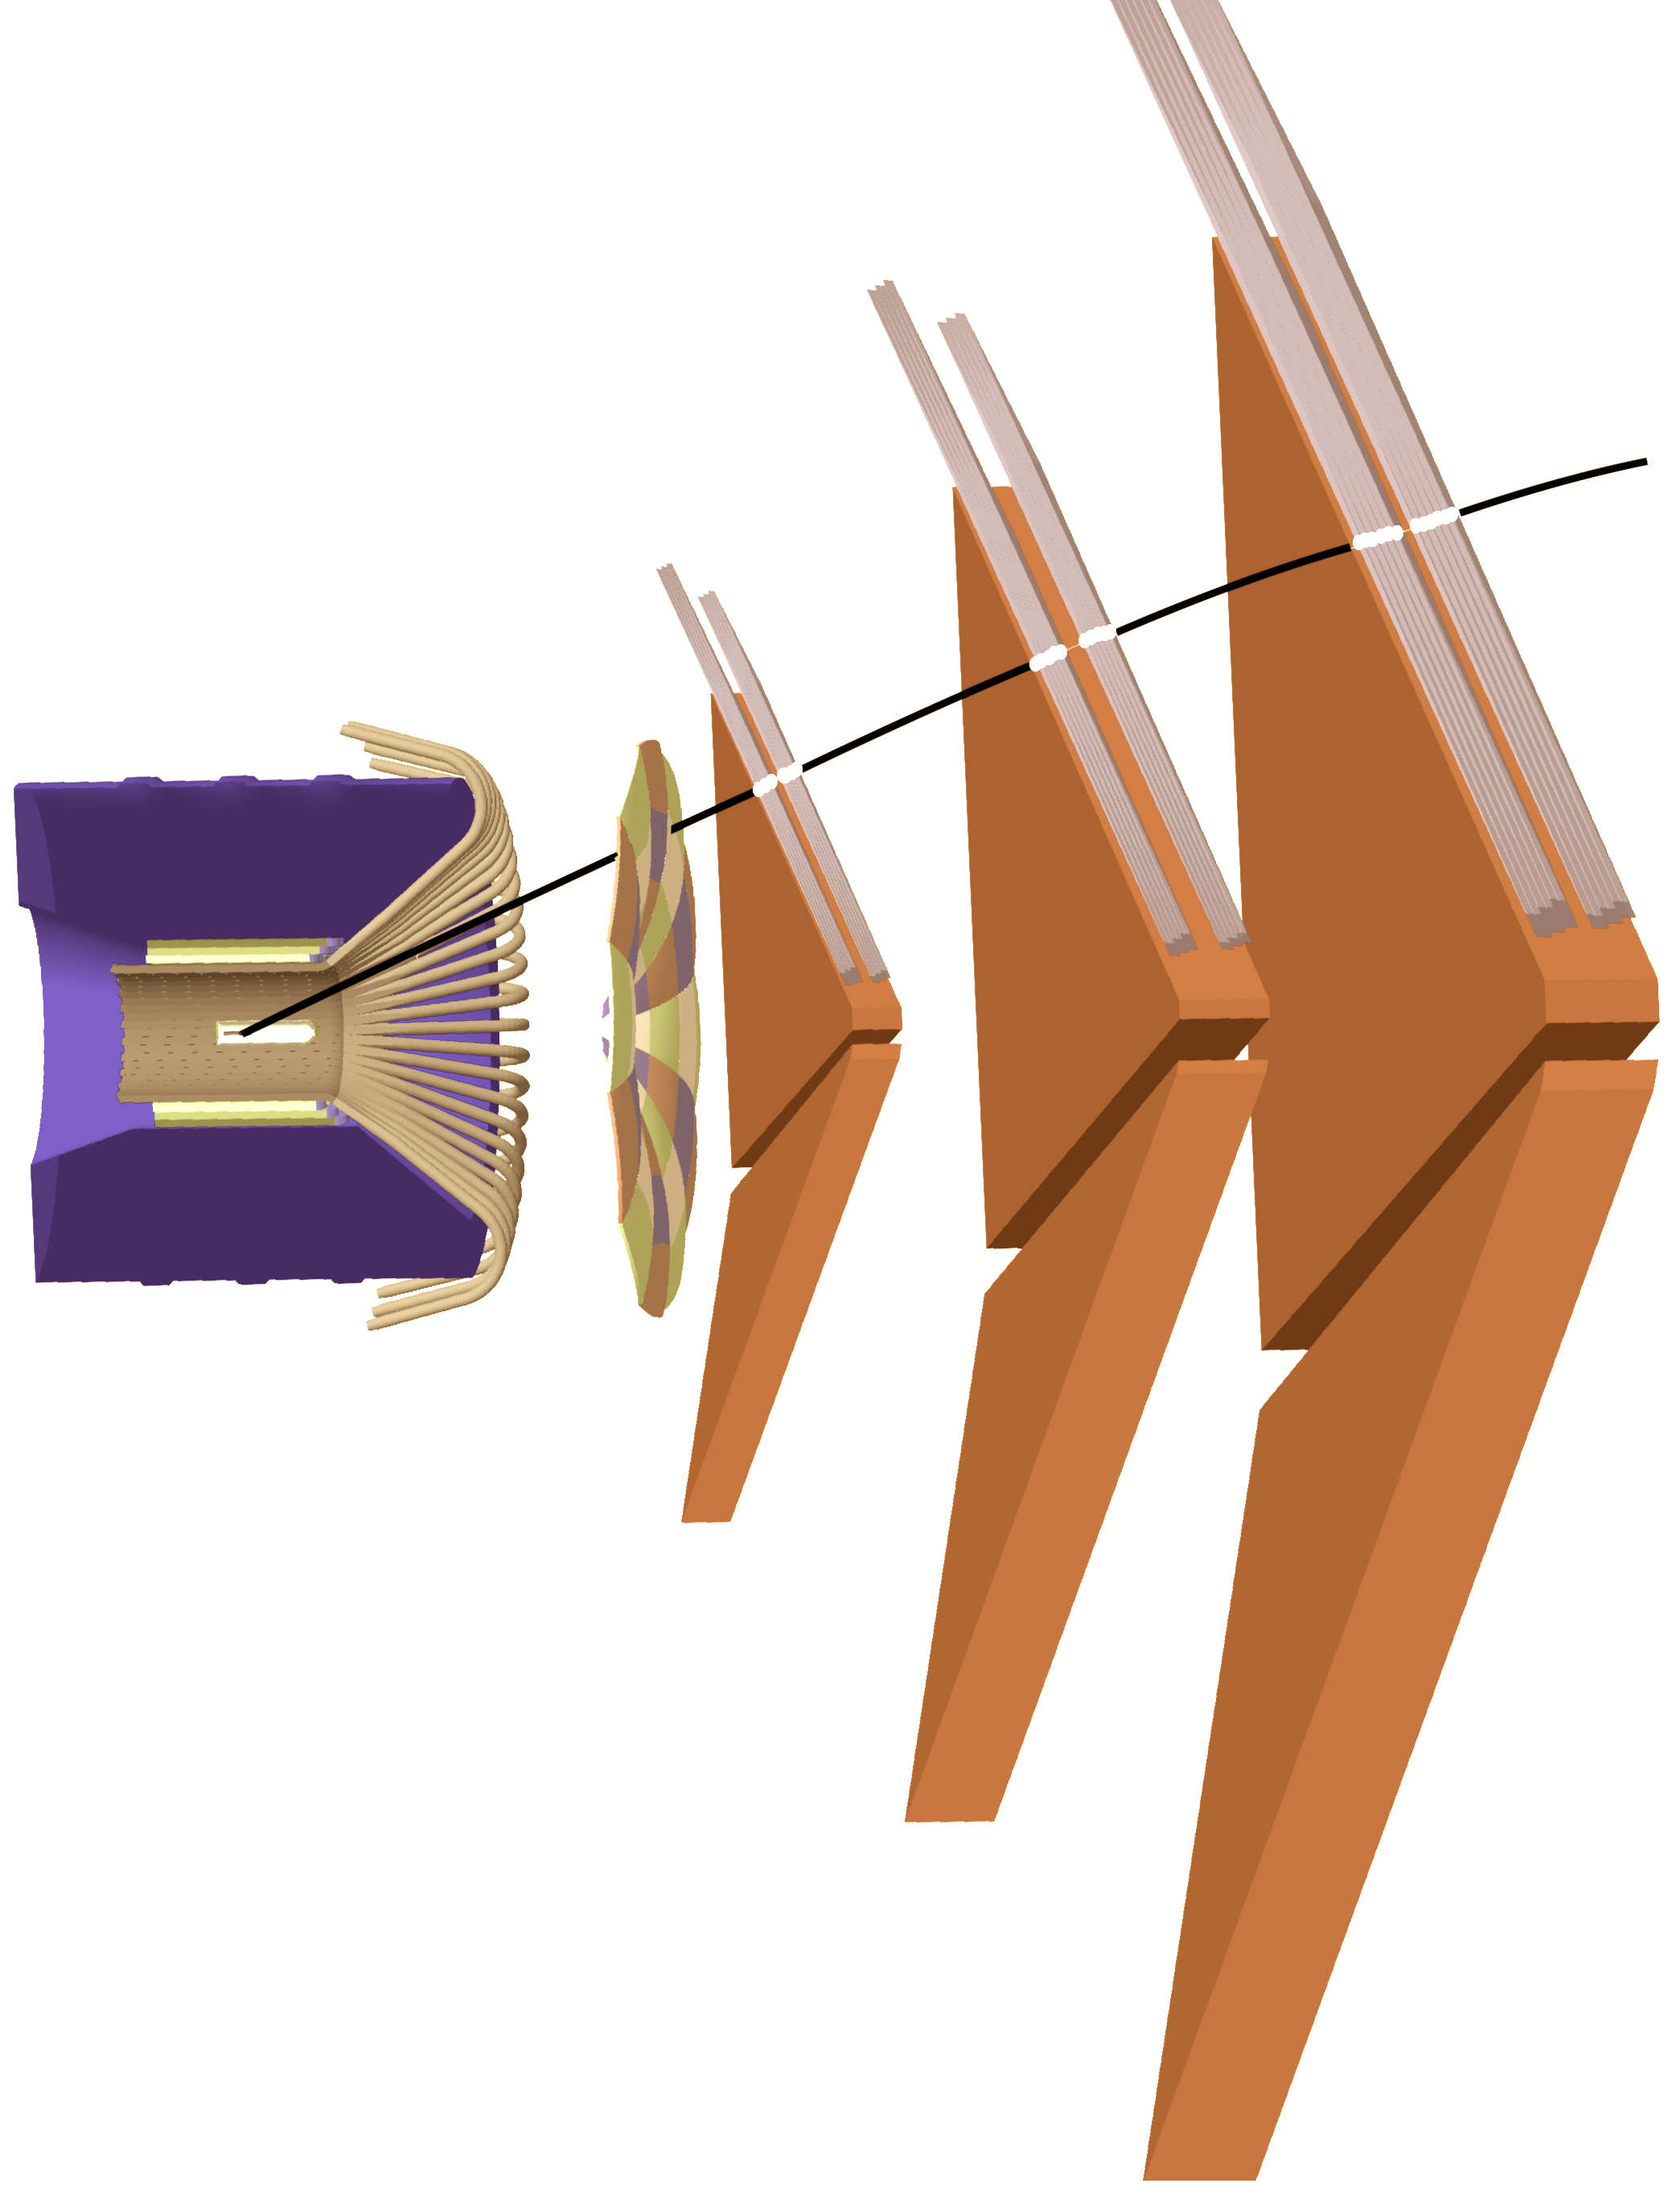
\includegraphics[width=0.95\columnwidth,keepaspectratio]{img/dcGeometry.png}
	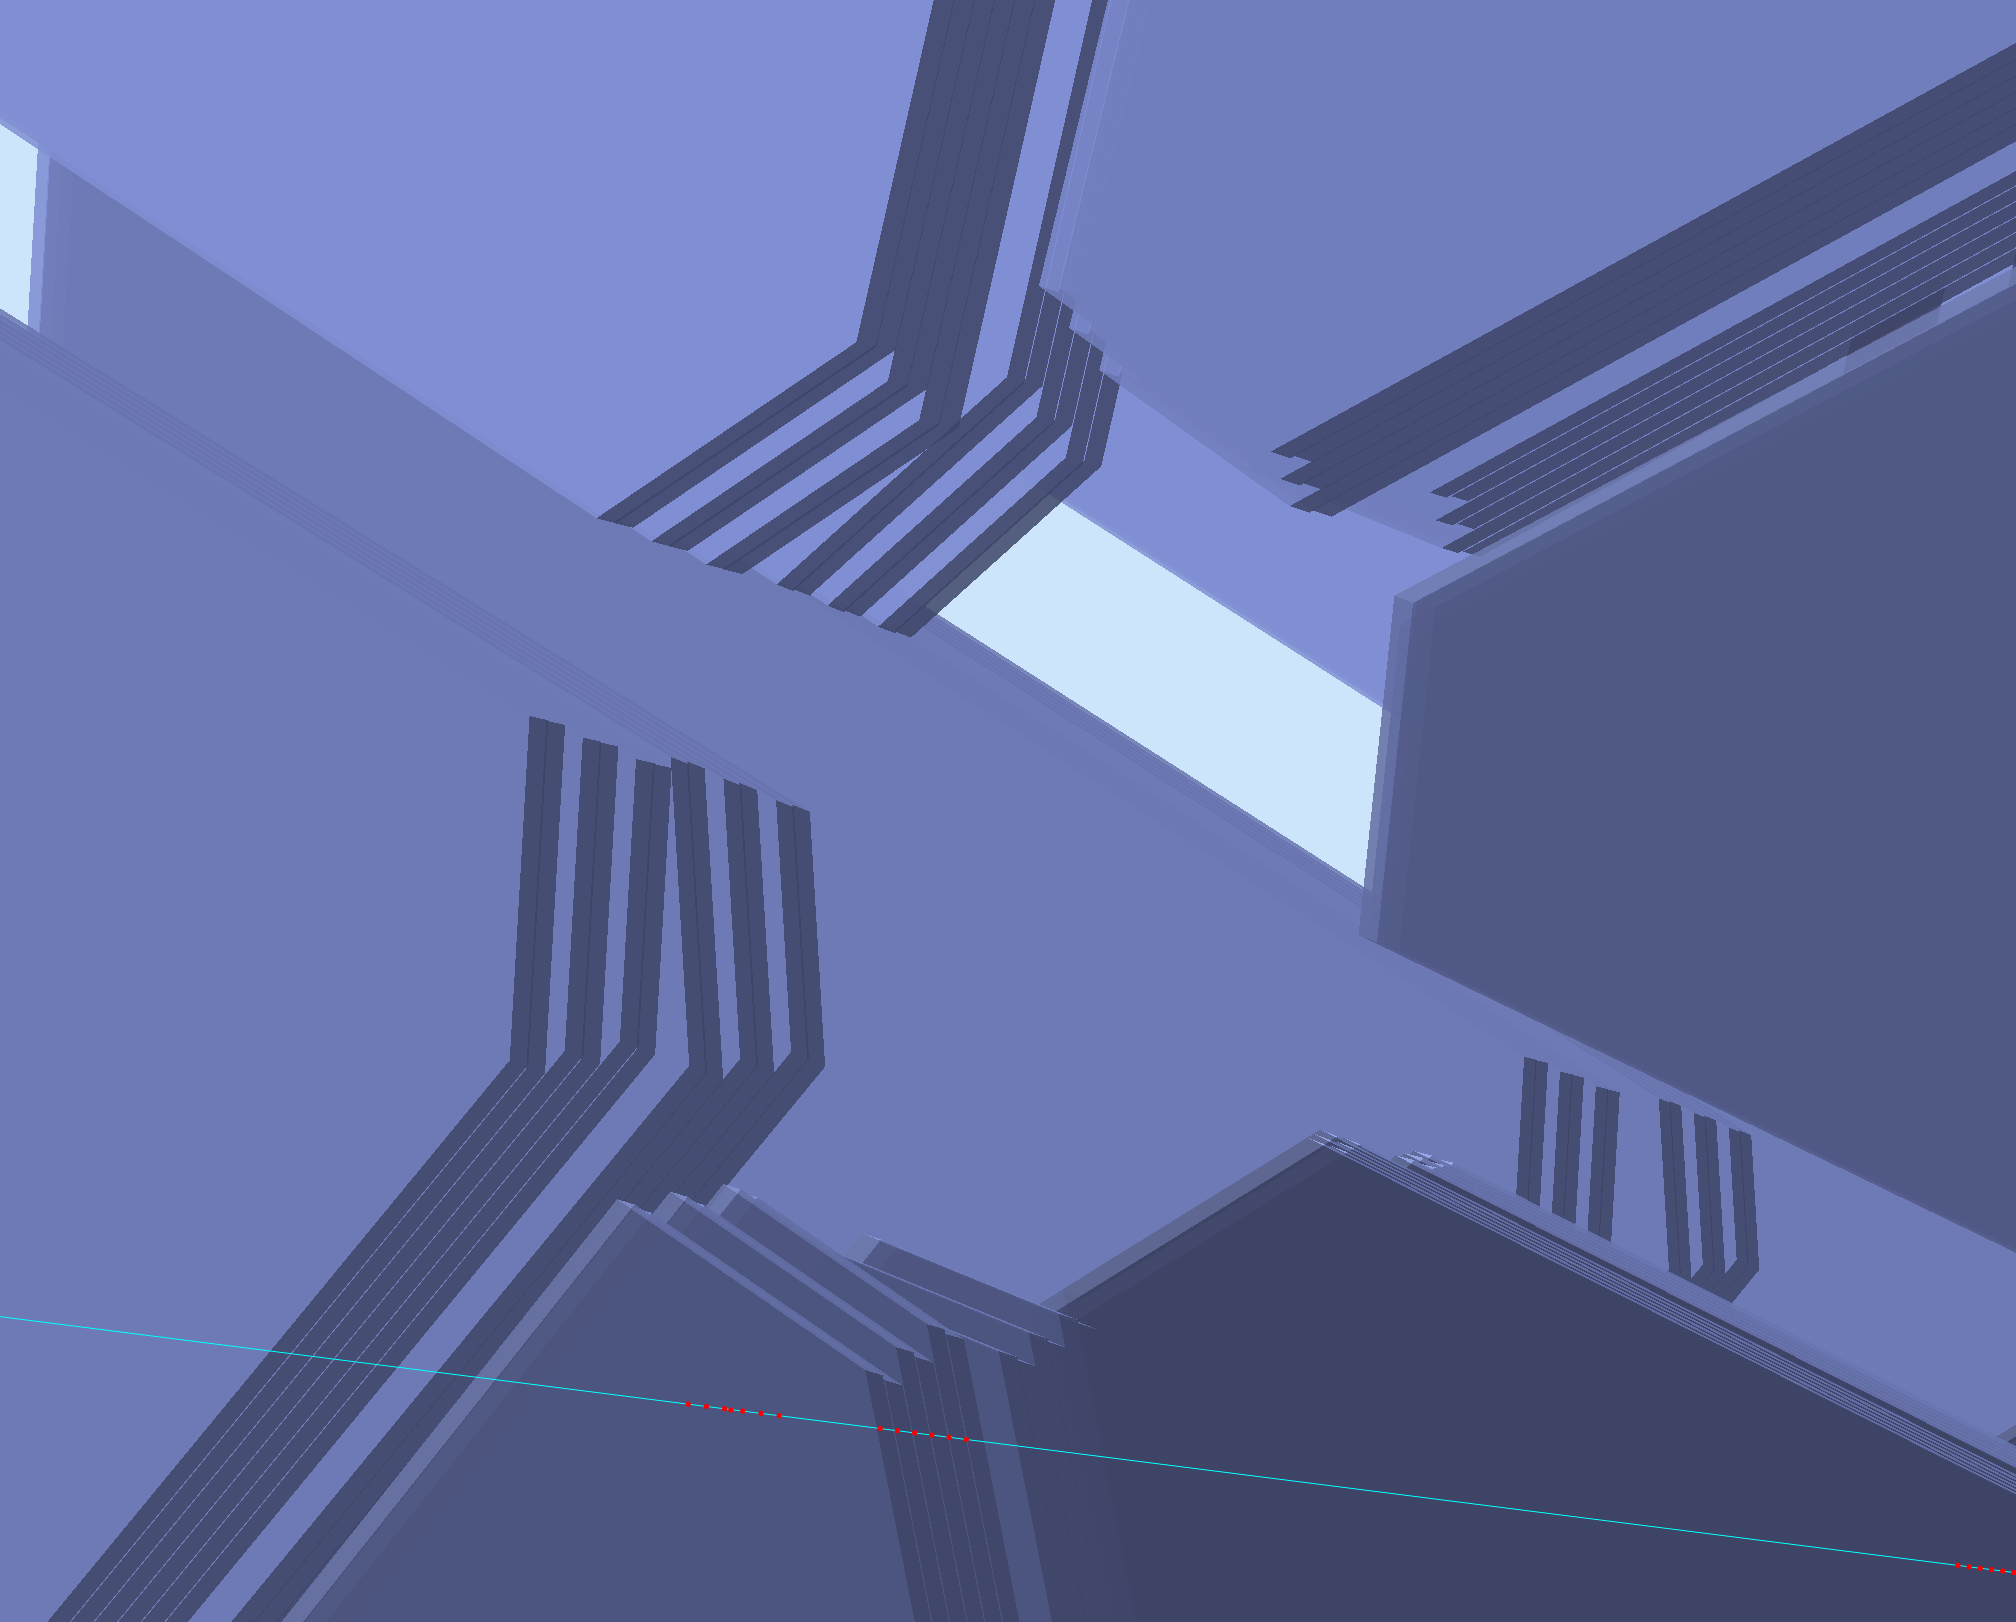
\includegraphics[width=0.95\columnwidth,keepaspectratio]{img/dcDetail.png}
	\caption{Top: the GEMC implementation of the FTOF geometry. The paddles are G4Boxes, embedded in trapezoid representing the mother volumes of each panel.
            Bottom: a zoom-in of the implementation shows the details of the individual paddles for Panel 1B (green) and Panel 1A (purple) }
	\label{fig:dcGeometry}
\end{figure}


\subsubsection{Geometry Git Location}

The github location of the gemc perl api script is \url{https://github.com/gemc/detectors/tree/master/clas12/dc}.
The geometry service definitions in coatjava is \url{https://github.com/JeffersonLab/clas12-offline-software/blob/development/common-tools/clas-jcsg/src/main/java/org/jlab/detector/geant4/v2/DCGeant4Factory.java}

\subsection{Process ID}
At each geant4 step, the local vertical position $y$ in the tilted g4Trap is computed. Knowing the distance
between each wire $\delta Y$ (given by the total height of the trapozoid divided by the number of wires, $112$), which is a constant as we're not taking into
account wire sagging, the wire ID is given by $n_i = y / \delta y$.


\subsection{Digitization}

\subsubsection{ADC}
There is no ADC calculation.

\subsubsection{TDC}
First, the distance of closest approach $DOCA$ is extrapolated for the hit. At each geant4 step, the distance of the track from the wire is calculated.
The $DOCA$ is extracted among the points with energy deposited greatr than $50 eV$, for which the sum of the step time + $DOCA / DV$ (where DV is the drift velocity) is minimal.

An initial time $T_i$ is calculated with a time to distance function which is the inverse of what extrapolated in calibration and used in reconstruction to go from TDC to $DOCA$.
The function takes into account:

\begin{itemize}
	\item the distance from the wire, in cm
	\item the cell size in superlayer
	\item the polar angle of the track
	\item magnitude of field in tesla
\end{itemize}

A time walk correction function is applied to $T_i$ that includes discrete ionisation effects based on the following input:

\begin{itemize}
	\item the distance from the wire, in cm
	\item the cell size in superlayer
	\item an adjustable factor (in mm) times $beta^2$ of the particle, the factor is adjusted according to data at small distances from the wire
	\item a parameter to adjust the matching between the two time walk distributions
	\item the velocity of the particle
\end{itemize}

The resulting $T_w$ is then used in a landau-function to mimic the detector response function.

An intrinsic random time walks correction $\sigma_{TW}$ due to multiple scattering is calculated and the time is smeared with
a gaussian function using $\sigma_{TW}$ as the resolution.

Finally, a random number is thrown and if it's above the efficiency function, calculated based on $DOCA$, the hit is rejected.


\subsubsection{Summary of CCDB Table used}
\begin{itemize}
	\item /calibration/dc/signal\_generation/intrinsic\_inefficiency
	\item /calibration/dc/signal\_generation/dc\_resolution
	\item /calibration/dc/time\_to\_distance/time2dist
	\item /geometry/dc/superlayer
\end{itemize}


\subsection{Digitized Bank}

\subsubsection{Time Window}

\subsubsection{Process Routine Git Repository Location}


The DC hit process routine location in git is \url{https://github.com/gemc/source/blob/master/hitprocess/clas12/dc_hitprocess.cc}
